\section{Auswertung}
\label{sec:Auswertung}
\subsection{Kalibrierung}
\begin{table}
  \caption{Länge der vom linken, bzw. rechten, Detektor ausgegebenen Impulse ohne Hinzuschalten eines Diskriminators}
  \label{tab:oD}
  \centering
  \begin{tabular}{|S|S|}
    \toprule
    $t_{links}/\si{\nano \second}$ & $t_{rechts}/\si{\nano \second}$\\
    \midrule
    6,6 & 10,2 \\
    8,6 & 7,8 \\
    8,2 & 10,4 \\
    10,0 & 7,6 \\
    14,0 & 9,4 \\
    9,0 & 11,8 \\
    10,6 & 8,4 \\
    8,6 & 12,0 \\
    10,4 & 7,6 \\
    11,0 & 10,0 \\
    \toprule
  \end{tabular}
\end{table}

Nach Hinzuschalten der Diskriminatoren beträgt $t_{links}= \SI{19,6}{\nano\second}$ und $t_{rechts} = \SI{19,0}{\nano \second}$. Die Diskriminatoren sind hierbei so aufeinander abgestimmt, dass sich ihre Ereignisfrequenzen nur um $\Delta_f = \SI{0,05}{\hertz}$ unterscheiden. Ihre Ereignisfrequenzen liegen bei $f_{links} = \SI{38.27}{\hertz}$, bzw. $f_{rechts}= \SI{38,22}{\hertz}$.

\begin{table}
  \caption{Nach der Koinzidenzschaltung registrierte Ereignisse in Abhängigkeit der relativen Verzögerung der Signale zueinander.}
  \label{tab:koinzidenz}
  \centering
  \begin{tabular}{|S|S|S|}
    \toprule
    $t_{VZ}/\si{\nano\second}$ & $\text{Ereignisse}$ & $\text{Messzeit}/\si{\second}$ \\
    \midrule
    0.0 & 421 & 20.22 \\
    16.0 & 422 & 21.39  \\
    20.0 & 285 & 20.20 \\
    22.0 & 174 & 20.24 \\
    23.0 & 116 & 19.96 \\
    23.5 & 85 & 20.06 \\
    -8.0 & 470 & 20.36 \\
    -40.0 & 14 & 20.45 \\
    8.0 & 441 & 19.98 \\
    12.0 & 451 & 20.05 \\
    -24.0 & 10  & 20.42 \\
    -28.0 & 10 & 20.42 \\
    -20.0 & 169 & 20.03 \\
    -22.0 & 63 & 20.16 \\
    -18.0 & 282 &20.30 \\
    -17.0 & 301 & 20.15 \\
    -19.0 & 211 & 20.40 \\
    -10.0 & 449 & 20.23 \\
    1.0 & 479 & 20.59 \\
    -12.0 & 426 & 20.10 \\
    0.0 & 463 20.05 \\
    \bottomrule
  \end{tabular}
\end{table}

Für die relative Verzögerungszeit $t_{VZ}= \SI{0.0}{\nano\second}$ wurden zwei Messwerte aufgenommen, da sie sich sehr nah am gemessenen Maximum von $t_{VZ}= \SI{1.0}{\nano\second}$ befindet und die erste Messung einen recht stark abweichenden Wert zeigt, obwohl ein ausgeprägtes Platau erwartet wird.


\begin{table}
  \caption{Unbearbeitete Messwerte zur Kalibrierung des Vielkanalanalysators}
  \centering
  \label{tab:kanal}
    \begin{tabular}{|S|S|S|}
      \hline
      $t/\si{\micro\second}$ & $\text{Kanal}$ & $\text{Counts}$ \\ \hline

      1 & 22 & 5055 \\
      1 & 23 & 999 \\ \hline
      2 & 44 & 196 \\
      2 & 45 & 4075 \\ \hline
      3 & 67 & 3815 \\ \hline
      4 & 89 & 4863 \\ \hline
      5 & 111 & 5904 \\ \hline
      6 & 133 & 5612 \\ \hline
      7 & 155 & 899 \\ \hline
      8 & 177 & 6509 \\ \hline
      9 & 200 & 7437 \\\hline
    \end{tabular}
\end{table}

\begin{table}
  \caption{Kanäle mit vom Doppelimpulsgenerator vorgegebenen Zeitintervallen sowie ihr Abstände}
  \label{tab:Kalibrierung}
  \centering
  \sisetup{round-mode = places , round-precision = 2,scientific-notation=fixed, fixed-exponent = 0}
  \begin{tabular}{|S|S|}
    \toprule
    $\text{Kanal}$ & $\text{Abstand}$ \\
    \midrule
    0.            &  \\
    22.16501487   & 22.16501487 \\
    44.95410911   & 22.78909424 \\
    67.           & 22.04589089 \\
    89.           & 22 \\
    111.          & 22 \\
    133.          & 22 \\
    155.          & 22 \\
    177.          & 22 \\
    199.          & 22 \\
    \bottomrule
  \end{tabular}
\end{table}

Aus den in Tab. \ref{tab:Kalibrierung} aufgeführten Werten (gemittelt aus Tab. \ref{tab:kanal} nach \eqref{eq:kanal}) ergibt sich eine Umrechnung von $(22.11 \pm 0.08) \, \frac{\text{Kanäle}}{\si{\micro\second}}$.

\subsection{Messung der Individuallebensdauern kosmischer Myonen}

\begin{figure}
  \centering
  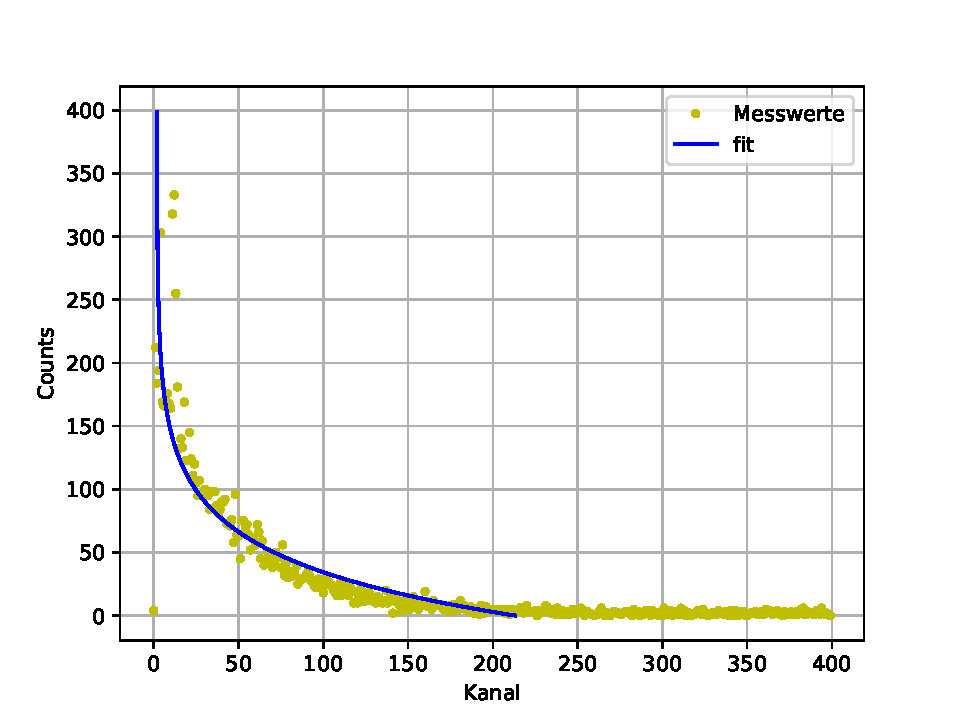
\includegraphics{./plots/lebensdauer.pdf}
  \caption{Gemessene Individuallebensdauern der detektierten Myonen}
  \label{fig:tau}
\end{figure}


Ein mittels $matplotlib$ \cite{matplotlib} über die Methode der kleinsten Quadrate durchgeführter Fit der Werte der Individuallebensdauern (dargestellt in Abb. \ref{fig:tau}) an eine Exponentialfunktion liefert folgende Werte:
\begin{align*}
  \tau &= \SI{2.03 \pm 0.09}{\micro\second} \\
  U &= 1.9 \pm 1.2 \\
  A &= 211 \pm 5
\end{align*}

Hierbei bezeichnet $U$ einen konstanten Untergrund aus zufällig, gleichverteilt auftretenden Ereignissen und $A$ als Ordinatenabschnitt.
Hierbei wurden die leeren ersten beiden Kanäle, sowie die ebenfalls leeren Kanäle 401 bis 511, bei der Auswertung der Daten vernachlässigt. Die ersten beiden Kanäle decken eine Zeit von ca. $t_{tot} = \SI{0.09}{\micro \second}$ ab.


% \begin{figure}
%   \centering
%   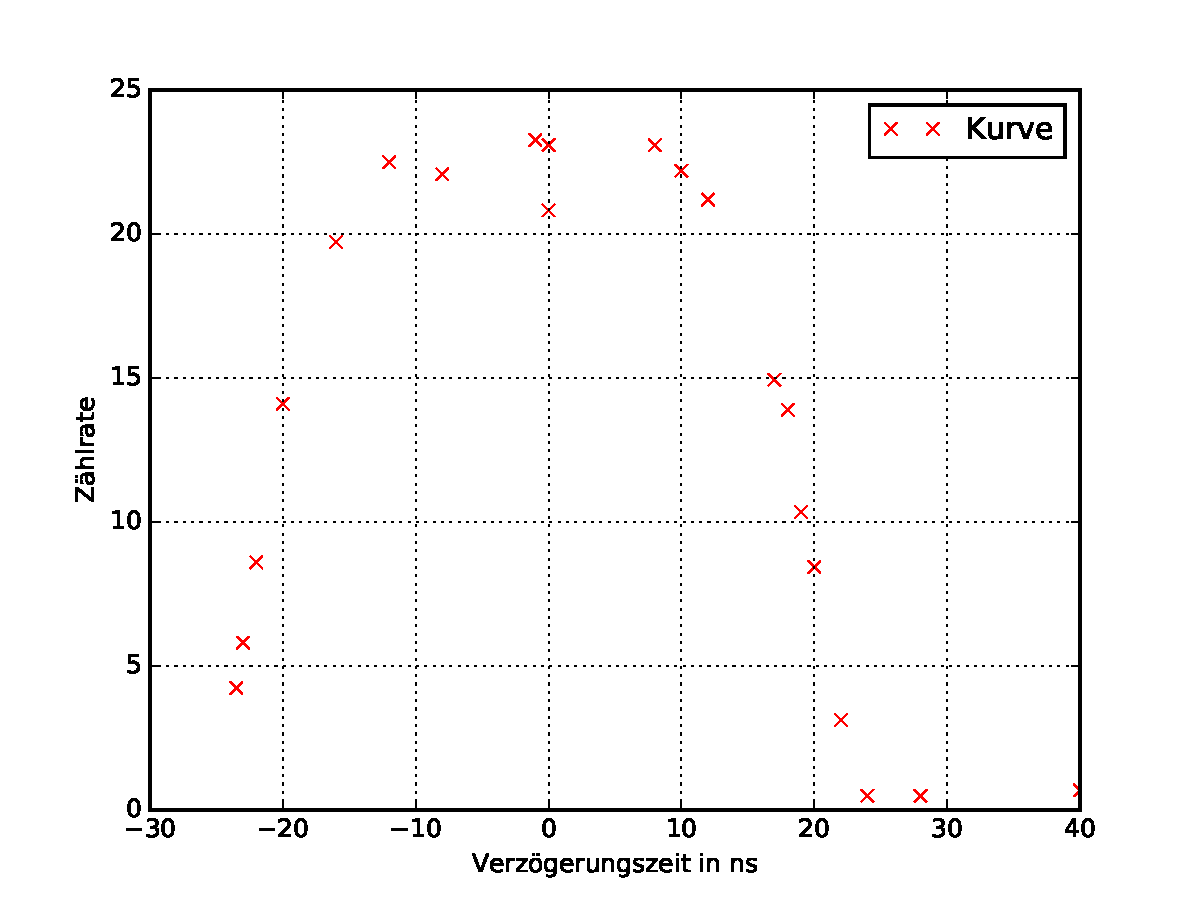
\includegraphics{plot.pdf}
%   \caption{Plot.}
%   \label{fig:plot}
% \end{figure}



% \begin{table}
%    % Notation :  {% nicht entfernen ist sehr wichtig sonst Fehler !!
% \parbox{0.48\textwidth}{% %Ermöglicht zwei Tabellen neben einander
%   \centering
%   \sisetup{round-mode = places , round-precision = 0,scientific-notation=fixed, fixed-exponent = 0}
%          %rundet Werte aus Stelle, Stelle = ,  macht einen bestimmten festen exponenten
%   \resizebox{\textwidth}{!}{%  % skaliert zu große Tabellen
%   \begin{tabular}{S@{${}\pm{}$} S} % fügt plus minus Fehler Schreibweise hinzu
%     \toprule
%      $\text{e}_b / \si{\milli\meter}$ &
%      $\text{d}_b /\si{\milli\meter} $ & $\text{f}_b / \si{\milli\meter} $\\
%     \midrule
%     \bottomrule
%   \end{tabular}
%   % }
%   \caption{Tabellenunterschrift}
%   \label{tab:tab}
% }
% % \end{table}
% % \begin{table}
% \parbox{0.48\textwidth}{%
%   \centering
%   \sisetup{round-mode = places , round-precision = 0,scientific-notation=fixed, fixed-exponent = 0}
%   % \resizebox{\textwidth}{!}{%
%   \begin{tabular}{S@{${}\pm{}$} S}
%     \toprule
%      $\text{e}_b / \si{\milli\meter}$ &
%      $\text{d}_b /\si{\milli\meter} $ & $\text{f}_b / \si{\milli\meter} $\\
%     \midrule
%     \bottomrule
%   \end{tabular}
%   % }
%   \caption{Tabellenunterschrift}
%   \label{tab:tab}
% }
% \end{table}
